\subsection{Background}
\begin{frame}

\begin{columns}
    \begin{column}{0.6\textwidth}
        \begin{itemize}
            \item Predicting the neutron flux distribution is crucial for reactor analysis
            \item The flux distribution determines the power distribution, which has important ramifications for design and operation
            \begin{itemize}
                \item Economically, efficient fuel loading patterns and prevention of fuel failures are determined largely by the power distribution
                \item The power distribution also drives safety constraints for both steady-state and transient operation, including accident scenarios
            \end{itemize}
            \item These requirements demand a high degree of accuracy from the codes used in reactor analysis
        \end{itemize}
    \end{column}
\begin{column}{0.4\textwidth}
\vfill
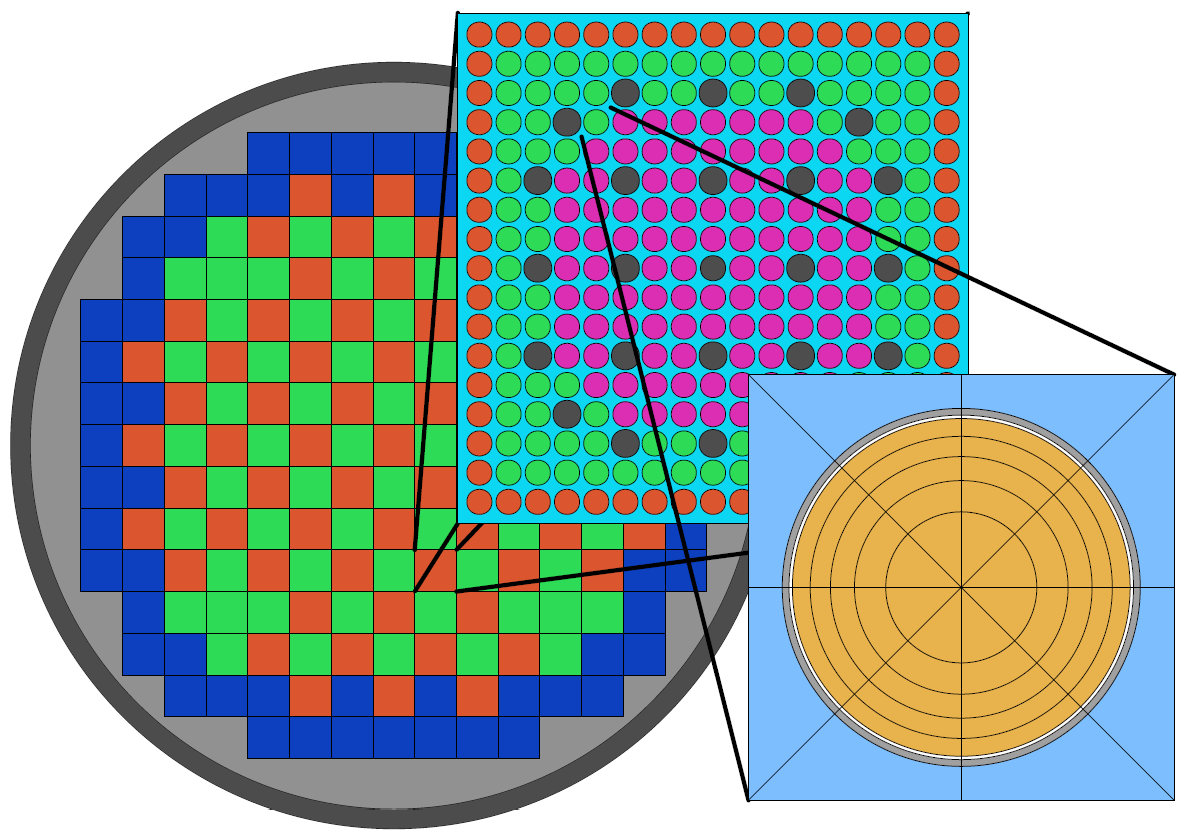
\includegraphics[width=\columnwidth]{reactor-geometry.png}
\vfil
\end{column}
\end{columns}
    
\end{frame}

%%%%%%%%%%%%%%%%%%%%%%%%%%%%%%%%%%%%%%%%%%%%%%%%%%%%%%%%%%%%%%%%%%%%%%%%%%%%%%%%%

\begin{frame}
    
\begin{columns}
    \begin{column}{0.5\textwidth}
        \begin{itemize}
            \item Reactor analysis has traditionally used a two-step approach
            \begin{itemize}
                \item Lattice calculations to generate homogenized cross sections
                \item Nodal diffusion methods to solve global problem with homogenized cross sections
            \end{itemize}
            \item Recent increases in computing power have generated interest in direct, whole-core transport calculations
            \begin{itemize}
                \item Monte Carlo
                \item Deterministic 3D transport
                \item Planar Synthesis Methods: 2D/1D and 2D/3D
            \end{itemize}
        \end{itemize}
    \end{column}
    \begin{column}{0.5\textwidth}
        \vfill
        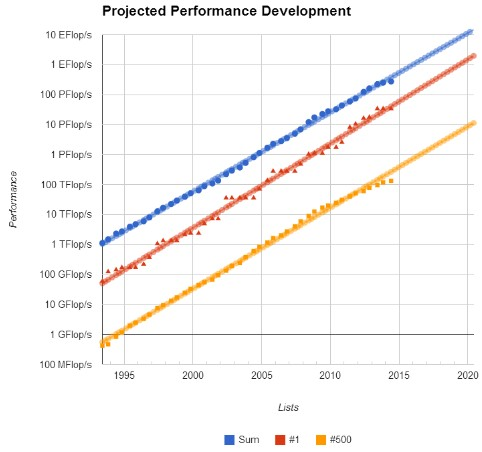
\includegraphics[width=\columnwidth]{top500-performance.jpg}
        \vfill
    \end{column}
\end{columns}

\end{frame}

%%%%%%%%%%%%%%%%%%%%%%%%%%%%%%%%%%%%%%%%%%%%%%%%%%%%%%%%%%%%%%%%%%%%%%%%%%%%%%%%

\begin{frame}

\begin{itemize}
    \item Monte Carlo
    \begin{itemize}
        \item Randomly samples cross sections to simulate the life of individual neutrons
        \item Simulating many neutrons can be used to describe average behavior of neutrons throughout reactor
        \item Prohibitively slow for large problems due to statistical uncertainties
    \end{itemize}
    \item Deterministic 3D transport
    \begin{itemize}
        \item Numerical methods are used to solve the transport equation in 3D
        \item Accurate solutions can be obtained
        \item Solving the transport equation can be too expensive for large problems
    \end{itemize}
    \item Planar Synthesis Methods
    \begin{itemize}
        \item Problem is decomposed into a stack of 2D planes, each assumed to be axially constant
        \item 2D transport equation is solved for each 2D plane, then coupled using a fast 1D solver (2D/1D) or 3D solver (2D/3D)
        \item Preserves much of the accuracy of 3D transport, but runs much faster
    \end{itemize}
\end{itemize}

\end{frame}

%%%%%%%%%%%%%%%%%%%%%%%%%%%%%%%%%%%%%%%%%%%%%%%%%%%%%%%%%%%%%%%%%%%%%%%%%%%%%%%%

\subsection{Motivation}
\begin{frame}[t]{Rod Cusping}

\begin{columns}
    \begin{column}{0.6\textwidth}
        \begin{itemize}
            \item Planar synthesis methods require planes to be axially homogeneous
            \item If any axial heterogeneities are present in the plane, they must be homogenized axially
            \item Volume homogenization is used since flux distribution is not yet known
            \item Control rods are strong neutron absorbers, causing the most severe homogenization errors
            \item Errors caused by rods partially inserted in a plane are called ``rod cusping''
        \end{itemize}
    \end{column}
    \begin{column}{0.4\textwidth}
        \begin{figure}[h]
            \centering
            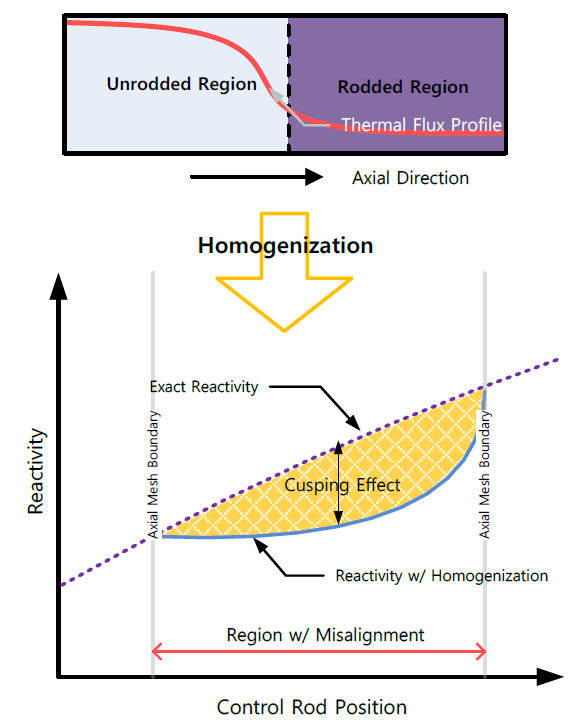
\includegraphics[width=\textwidth]{cusping_effect_Joo.png}
        \end{figure} 
    \end{column}
\end{columns}

\end{frame}

%%%%%%%%%%%%%%%%%%%%%%%%%%%%%%%%%%%%%%%%%%%%%%%%%%%%%%%%%%%%%%%%%%%%%%%%%%%%%%%%%

\begin{frame}
    
    \begin{itemize}
        \item Planar synthesis methods are faster than 3D transport, but still computationally expensive
        \item To make these methods useful practically, runtimes need to be decreased
        \begin{itemize}
            \item Algorithm and methods improvements
            \item Reduction in number of planes
        \end{itemize}
        \item Subgrid methods can be used to maintain accuracy with fewer planes by loosening requirement that planes be axially homogeneous
        \begin{itemize}
            \item Needs to be able to capture local effects of various reactor components
            \item Should be able to be applied to a variety of situations
            \item Cheaper than using more planes
        \end{itemize}
        \item Three new methods developed to accomplish two goals:
        \begin{itemize}
            \item Significant reduction in errors caused by rod cusping, the most severe axial heterogeneity for planar synthesis methods
            \item Reduce the runtime of the 2D/1D code MPACT by using fewer planes
        \end{itemize}
    \end{itemize}

\end{frame}